\chapter{Propagation Modes: Ground Wave, Sky Wave, and Line-of-Sight}
\label{ch:propagation-modes}

\begin{nontechnical}
\textbf{Radio waves can travel three different ways}---think of it like: rolling on the ground, bouncing off the sky, or shooting straight like a laser!

\textbf{1. Ground Wave (Surface Wave)}
\begin{itemize}
\item \textbf{What:} Radio wave hugs the Earth's surface and bends around the curve
\item \textbf{Frequency:} Low (AM radio, 500~kHz--1.5~MHz)
\item \textbf{Range:} 100--1000+~km depending on frequency
\item \textbf{Analogy:} Rolling a ball on the ground---it follows the terrain
\end{itemize}

\textbf{Real examples:}
\begin{itemize}
\item \textbf{AM radio stations:} Travel hundreds of miles, even over the horizon
\item \textbf{Maritime communications:} Ships use ground wave to communicate over the ocean
\end{itemize}

\textbf{2. Sky Wave (Ionospheric Bounce)}
\begin{itemize}
\item \textbf{What:} Radio wave shoots up, bounces off ionosphere (layer of charged particles 100--400~km up), comes back down
\item \textbf{Frequency:} Medium (shortwave radio, 3--30~MHz / HF)
\item \textbf{Range:} Global! Can bounce multiple times
\item \textbf{Analogy:} Skipping a stone on water---one throw, many bounces
\end{itemize}

\textbf{Real examples:}
\begin{itemize}
\item \textbf{Shortwave radio:} Broadcast from London, heard in Australia!
\item \textbf{Amateur (ham) radio:} Talk to people on other continents
\item \textbf{Why it works at night:} Ionosphere gets stronger after sunset
\end{itemize}

\textbf{3. Line-of-Sight (LOS)}
\begin{itemize}
\item \textbf{What:} Radio wave travels straight like light---if you can't ``see'' the tower, signal is blocked
\item \textbf{Frequency:} High (FM radio, TV, cell phones, WiFi, 30~MHz+)
\item \textbf{Range:} Limited to visible horizon ($\sim$5--50~km depending on height)
\item \textbf{Analogy:} Laser pointer---must have clear path
\end{itemize}

\textbf{Real examples:}
\begin{itemize}
\item \textbf{Cell phones:} Need tower in view (mostly)
\item \textbf{WiFi:} Walls/floors block it
\item \textbf{Satellite TV:} Dish must point directly at satellite (trees in the way = no signal!)
\item \textbf{5G mmWave:} Can't even go through your hand!
\end{itemize}

\textbf{Why different modes?}
\begin{itemize}
\item \textbf{Lower frequency} $\rightarrow$ bends around obstacles, long range, slow data
\item \textbf{Higher frequency} $\rightarrow$ straight-line only, shorter range, fast data
\end{itemize}

\textbf{Fun fact:} During the Cold War, governments used sky wave propagation to broadcast radio into other countries---signals would bounce off the ionosphere and arrive ``from above,'' impossible to block!
\end{nontechnical}

\section{Overview}

Electromagnetic waves propagate via different mechanisms depending on frequency, distance, and environment. Understanding propagation modes is essential for predicting coverage and designing wireless systems.

\begin{keyconcept}
The propagation mode is primarily determined by \textbf{frequency}. Low frequencies (LF/MF) follow Earth's curvature via ground wave, high frequencies (HF) bounce off the ionosphere via sky wave, and very high frequencies (VHF+) require direct line-of-sight paths.
\end{keyconcept}

\textbf{Three primary modes:}
\begin{enumerate}
\item \textbf{Ground Wave} (Surface wave) -- LF/MF/HF, follows Earth's curvature
\item \textbf{Sky Wave} (Ionospheric) -- HF, bounces off ionosphere, global reach
\item \textbf{Line-of-Sight (LOS)} -- VHF and above, direct path required
\end{enumerate}

\subsection{Propagation Mode Visualization}

Figure~\ref{fig:propagation-modes} illustrates the three primary propagation modes and their characteristics.

\begin{figure}[htbp]
\centering
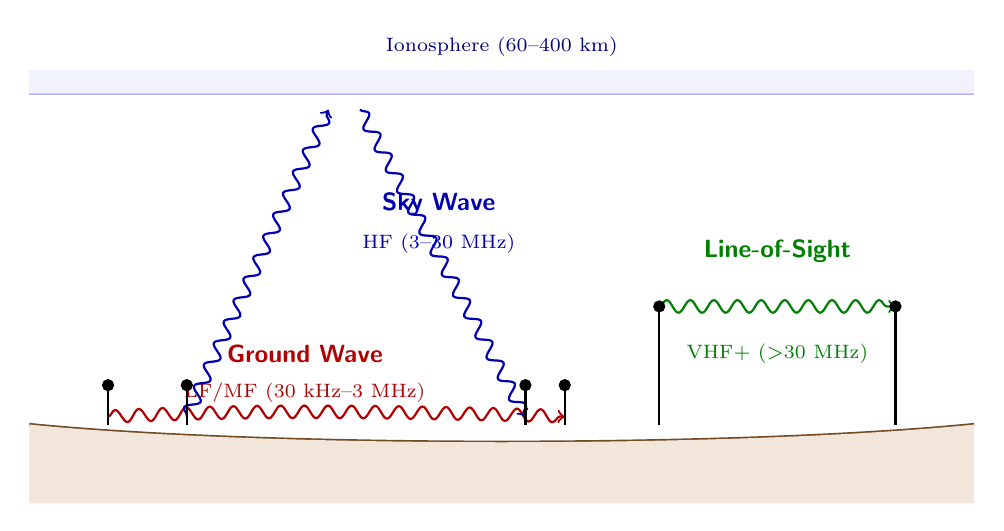
\begin{tikzpicture}[scale=1.0, font=\small]
% Earth surface (curved)
\draw[very thick, brown!60!black] (-6,0) .. controls (-3,-0.3) and (3,-0.3) .. (6,0);
\fill[brown!20] (-6,0) .. controls (-3,-0.3) and (3,-0.3) .. (6,0) -- (6,-1) -- (-6,-1) -- cycle;

% Ground Wave
\draw[->, thick, red!70!black, decorate, decoration={snake, amplitude=0.8mm, segment length=3mm}] 
  (-5,0.1) .. controls (-3,0.2) and (-1,0.15) .. (0.8,0.1);
\node[red!70!black, font=\sffamily\small] at (-2.5,0.9) {\textbf{Ground Wave}};
\node[red!70!black, font=\scriptsize] at (-2.5,0.4) {LF/MF (30 kHz--3 MHz)};

% Sky Wave - Ionosphere layer
\draw[blue!30, thick] (-6,4.2) -- (6,4.2);
\fill[blue!10, opacity=0.5] (-6,4.2) rectangle (6,4.5);
\node[blue!50!black, font=\scriptsize] at (0,4.8) {Ionosphere (60--400 km)};

% Sky Wave path
\draw[->, thick, blue!70!black, decorate, decoration={snake, amplitude=0.8mm, segment length=3mm}] 
  (-4,0.1) -- (-2.2,4.0);
\draw[->, thick, blue!70!black, decorate, decoration={snake, amplitude=0.8mm, segment length=3mm}] 
  (-1.8,4.0) -- (0.3,0.1);
\node[blue!70!black, font=\sffamily\small] at (-0.8,2.8) {\textbf{Sky Wave}};
\node[blue!70!black, font=\scriptsize] at (-0.8,2.3) {HF (3--30 MHz)};

% Line-of-Sight
\draw[->, thick, green!50!black, decorate, decoration={snake, amplitude=0.8mm, segment length=3mm}] 
  (2,1.5) -- (5,1.5);
\node[green!50!black, font=\sffamily\small] at (3.5,2.2) {\textbf{Line-of-Sight}};
\node[green!50!black, font=\scriptsize] at (3.5,0.9) {VHF+ ($>$30 MHz)};

% Antennas - Ground Wave
\draw[thick] (-5,0) -- (-5,0.5);
\filldraw[black] (-5,0.5) circle (2pt);
\draw[thick] (-4,0) -- (-4,0.5);
\filldraw[black] (-4,0.5) circle (2pt);
\draw[thick] (0.8,0) -- (0.8,0.5);
\filldraw[black] (0.8,0.5) circle (2pt);

% Antennas - Sky Wave
\draw[thick] (0.3,0) -- (0.3,0.5);
\filldraw[black] (0.3,0.5) circle (2pt);

% Antennas - Line-of-Sight
\draw[thick] (2,0) -- (2,1.5);
\filldraw[black] (2,1.5) circle (2pt);
\draw[thick] (5,0) -- (5,1.5);
\filldraw[black] (5,1.5) circle (2pt);

\end{tikzpicture}
\caption{Three primary electromagnetic wave propagation modes: ground wave following Earth's surface, sky wave reflecting from ionosphere, and line-of-sight direct path.}
\label{fig:propagation-modes}
\end{figure}

\section{Ground Wave Propagation}
\label{sec:ground-wave}

\subsection{Definition}

A \textbf{ground wave} is an electromagnetic wave that travels along Earth's surface, guided by the ground-air interface.

\textbf{Mechanism:}
\begin{itemize}
\item Electric field induces currents in ground (conductive surface)
\item Ground acts as imperfect dielectric, slows wave slightly
\item \textbf{Diffraction} allows wave to follow Earth's curvature (beyond horizon)
\end{itemize}

\begin{calloutbox}{Frequency Range}
Ground waves are effective in the \textbf{LF to MF} bands (30~kHz--3~MHz), with limited use in \textbf{HF} (3--30~MHz). Higher frequencies experience severe attenuation.
\end{calloutbox}

\subsection{Attenuation Factors}

Ground wave attenuation depends on four key factors:

\begin{enumerate}
\item \textbf{Frequency:} Higher frequency = more attenuation
\item \textbf{Ground conductivity:} Seawater (high $\sigma$) $<$ freshwater $<$ wet soil $<$ dry soil $<$ ice
\item \textbf{Distance:} Exponential decay with range
\item \textbf{Polarization:} \textbf{Vertical polarization required} (horizontal is rapidly attenuated)
\end{enumerate}

\begin{warningbox}{Polarization Requirement}
Ground wave propagation \textbf{requires vertical polarization}. Horizontally polarized waves induce currents parallel to the ground surface and are rapidly attenuated. This is why AM broadcast antennas are always vertically oriented.
\end{warningbox}

\subsubsection{Ground Conductivity}

Table~\ref{tab:ground-conductivity} shows how different surface types affect ground wave attenuation.

\begin{table}[htbp]
\centering
\caption{Ground conductivity and attenuation for different surface types}
\label{tab:ground-conductivity}
\begin{tabular}{@{}lp{2.5cm}p{2.5cm}p{2.5cm}@{}}
\toprule
\textbf{Surface Type} & \textbf{Conductivity (S/m)} & \textbf{Relative Permittivity $\epsilon_r$} & \textbf{Attenuation} \\
\midrule
Seawater & 5 & 80 & \textbf{Very low} (best) \\
Freshwater & 0.01 & 80 & Low \\
Wet soil & 0.01--0.001 & 20--30 & Moderate \\
Dry soil & 0.001 & 3--10 & High \\
Urban/concrete & 0.001 & 5 & High \\
Ice/snow & 0.0001 & 3 & Very high \\
\bottomrule
\end{tabular}
\end{table}

\textbf{Maritime advantage:} Ships can communicate over 1000+~km at LF/MF (AM broadcast)

\textbf{Desert disadvantage:} Dry sand severely limits ground wave (100s of meters)

\subsection{Range vs Frequency}

Empirical range over average soil with vertical polarization is shown in Table~\ref{tab:ground-wave-range}.

\begin{table}[htbp]
\centering
\caption{Ground wave range vs frequency over average soil}
\label{tab:ground-wave-range}
\begin{tabular}{@{}lllp{4.5cm}@{}}
\toprule
\textbf{Frequency} & \textbf{Wavelength} & \textbf{Typical Range} & \textbf{Applications} \\
\midrule
50~kHz (VLF) & 6000~m & 500--1000~km & Navigation (LORAN) \\
150~kHz (LF) & 2000~m & 300--800~km & Longwave broadcast \\
500~kHz (MF) & 600~m & 200--500~km & Marine distress (SOS) \\
1~MHz (AM) & 300~m & 100--300~km & AM radio (nighttime skywave extends this) \\
3~MHz (HF) & 100~m & 10--50~km & Limited ground wave, skywave dominant \\
\bottomrule
\end{tabular}
\end{table}

\begin{importantbox}{Key Insight}
Ground wave range \textbf{decreases rapidly with frequency}. This is why low-frequency bands (LF/MF) are preferred for long-range ground wave communication.
\end{importantbox}

\subsection{Path Loss Model}

The \textbf{Norton ground wave equation} (simplified) gives the total path loss:

\begin{equation}
\label{eq:ground-wave-loss}
L_{\text{ground}} = L_{\text{FS}} + A_{\text{ground}}(f, d, \sigma, \epsilon_r)
\end{equation}

where:
\begin{itemize}
\item $L_{\text{FS}}$ = Free-space path loss (dB)
\item $A_{\text{ground}}$ = Additional ground attenuation (dB)
\item $f$ = Frequency (MHz)
\item $d$ = Distance (km)
\item $\sigma$ = Ground conductivity (S/m)
\item $\epsilon_r$ = Relative permittivity
\end{itemize}

For the MF band over average soil, an approximation is:

\begin{equation}
\label{eq:ground-attenuation}
A_{\text{ground}} \approx 0.1 \times \left(\frac{f}{1\text{ MHz}}\right)^2 \times \left(\frac{d}{1\text{ km}}\right) \quad \text{(dB)}
\end{equation}

\textbf{Example:} For 1~MHz at 100~km over average soil:
\begin{equation}
A_{\text{ground}} \approx 0.1 \times 1^2 \times 100 = 10\text{ dB additional loss}
\end{equation}

\subsection{Ground Wave Applications}

\subsubsection{AM Radio (540--1600~kHz)}

\textbf{Daytime:} Ground wave only
\begin{itemize}
\item Local coverage: 50--150~km
\item Limited by ground conductivity
\end{itemize}

\textbf{Nighttime:} Skywave + ground wave
\begin{itemize}
\item Extended coverage: 500--2000+~km (skywave reflection)
\item Interference common (multiple stations bounce off ionosphere)
\end{itemize}

\subsubsection{Maritime Communications (LF/MF)}

\textbf{VLF (20--100~kHz):} Submarine communications
\begin{itemize}
\item Penetrates seawater (10--20~m depth)
\item Global coverage (ground wave over ocean)
\item Very low data rate ($<$100~bps)
\end{itemize}

\textbf{MF (300--3000~kHz):} Ship-to-shore
\begin{itemize}
\item 200--500~km range over seawater
\item Distress frequency: 500~kHz (historical SOS)
\end{itemize}

\subsubsection{Aviation NDB (Non-Directional Beacons)}

\begin{itemize}
\item \textbf{Frequency:} 190--535~kHz
\item \textbf{Range:} 50--100~km (ground wave)
\item \textbf{Use:} Aircraft homing (ADF receivers)
\end{itemize}

\section{Sky Wave (Ionospheric Propagation)}
\label{sec:sky-wave}

\subsection{Definition}

A \textbf{sky wave} is an electromagnetic wave refracted by the ionosphere, returning to Earth at a distant location.

\textbf{Mechanism:}
\begin{enumerate}
\item HF wave travels upward at an angle
\item Ionosphere (charged plasma layer, 60--400~km altitude) acts as refractive medium
\item Wave bends back toward Earth (if frequency/angle correct)
\item Can bounce multiple times (multi-hop)
\end{enumerate}

\begin{calloutbox}{Frequency Range}
Sky waves are effective primarily in the \textbf{HF band (3--30~MHz)}, with some \textbf{MF propagation at night} when the D-layer disappears.
\end{calloutbox}

\subsection{Ionospheric Layers}

The ionosphere is ionized by solar UV and X-rays, creating distinct layers with different properties shown in Table~\ref{tab:ionospheric-layers}.

\begin{table}[htbp]
\centering
\caption{Ionospheric layers and their characteristics}
\label{tab:ionospheric-layers}
\small
\begin{tabular}{@{}llp{3.5cm}p{3.5cm}@{}}
\toprule
\textbf{Layer} & \textbf{Altitude} & \textbf{Daytime Behavior} & \textbf{Nighttime Behavior} \\
\midrule
\textbf{D} & 60--90~km & \textbf{Absorbs HF} (attenuates MF/HF) & \textbf{Disappears} (recombination fast) \\
\textbf{E} & 90--150~km & Reflects some HF ($<$10~MHz) & Weakens \\
\textbf{F1} & 150--250~km & Reflects MF/HF & \textbf{Merges with F2} \\
\textbf{F2} & 250--400~km & \textbf{Primary reflector} for HF & Descends, remains strong \\
\bottomrule
\end{tabular}
\end{table}

\begin{keyconcept}
The \textbf{critical frequency} $f_c$ is the maximum frequency reflected at vertical incidence, given by:
\begin{equation}
\label{eq:critical-frequency}
f_c = 9\sqrt{N_e}
\end{equation}
where $N_e$ is the electron density (electrons/m$^3$).
\end{keyconcept}

\textbf{Typical values:}
\begin{itemize}
\item Daytime F2 layer: $f_c = 10$--15~MHz
\item Nighttime F2 layer: $f_c = 5$--10~MHz
\end{itemize}

\subsection{Skip Distance and Hop}

The \textbf{skip distance} is the minimum ground range for sky wave return:

\begin{equation}
\label{eq:skip-distance}
d_{\text{skip}} = 2h\tan(\theta)
\end{equation}

where:
\begin{itemize}
\item $h$ = Ionospheric layer height (km)
\item $\theta$ = Elevation angle of departure (degrees)
\end{itemize}

\textbf{For F2 layer} ($h \approx 300$~km):
\begin{itemize}
\item Low angle (5°): Skip $\sim$3500~km (single hop)
\item High angle (45°): Skip $\sim$600~km
\end{itemize}

\begin{importantbox}{Dead Zone}
The \textbf{dead zone} is the region between the ground wave limit and skip distance where \textbf{no coverage} exists. This gap occurs because the ground wave has faded and the sky wave hasn't returned to Earth yet.
\end{importantbox}

\subsection{Multi-Hop Propagation}

The wave bounces between ionosphere and ground:

\begin{itemize}
\item \textbf{Single hop:} 2000--4000~km
\item \textbf{Two hops:} 4000--8000~km
\item \textbf{Multiple hops:} Global coverage possible (with sufficient power)
\end{itemize}

\textbf{Loss per hop:} 5--15~dB (depends on ionospheric conditions and frequency)

\subsection{Frequency Selection}

\textbf{MUF (Maximum Usable Frequency)} is the highest frequency that refracts back without penetrating the ionosphere:

\begin{equation}
\label{eq:muf}
\text{MUF} = \frac{f_c}{\cos(\theta)}
\end{equation}

where $f_c$ is the critical frequency and $\theta$ is the elevation angle.

\begin{itemize}
\item \textbf{LUF (Lowest Usable Frequency):} Lowest frequency not absorbed by D-layer
\item \textbf{Optimal Working Frequency (FOT):} 80--90\% of MUF (safety margin)
\end{itemize}

\subsection{Diurnal Variations}

\textbf{Daytime:}
\begin{itemize}
\item D-layer absorbs lower HF ($<$5~MHz)
\item F2 layer reflects higher HF (10--30~MHz)
\item \textbf{Best bands:} 15~MHz, 20~MHz (long-distance)
\end{itemize}

\textbf{Nighttime:}
\begin{itemize}
\item D-layer disappears (no absorption)
\item F2 descends, lower MUF
\item \textbf{Best bands:} 5~MHz, 7~MHz (medium-distance)
\item AM broadcast skywave active (500--1600~kHz)
\end{itemize}

\subsection{Seasonal and Solar Cycle Effects}

\textbf{Solar cycle (11 years):}
\begin{itemize}
\item \textbf{Solar max:} High ionization, higher MUF (30~MHz+ usable)
\item \textbf{Solar min:} Lower MUF (often $<$20~MHz)
\end{itemize}

\textbf{Seasonal:}
\begin{itemize}
\item \textbf{Summer:} Higher D-layer absorption (daytime)
\item \textbf{Winter:} Lower absorption, better long-distance (daytime)
\end{itemize}

\textbf{Sporadic E (Es):}
\begin{itemize}
\item Unpredictable intense E-layer patches
\item Reflects VHF (up to 150~MHz!) for short periods
\item Used opportunistically by amateur radio
\end{itemize}

\subsection{Sky Wave Applications}

\subsubsection{Shortwave Broadcast}

\begin{itemize}
\item \textbf{Frequency:} 3--30~MHz (HF bands)
\item \textbf{Range:} 500--10,000+~km (multi-hop)
\item \textbf{Use:} International broadcasting (BBC World Service, Voice of America)
\item \textbf{Schedule management:} Different frequencies for day/night and seasons
\end{itemize}

\subsubsection{Amateur Radio (Ham Radio)}

\begin{itemize}
\item \textbf{HF bands:} 1.8, 3.5, 7, 10, 14, 18, 21, 24, 28~MHz
\item \textbf{Activity:} Global communication with $<$100~W (due to skywave)
\item \textbf{80m (3.5~MHz):} Nighttime, regional (500--2000~km)
\item \textbf{20m (14~MHz):} Daytime, worldwide (DX)
\end{itemize}

\subsubsection{Over-the-Horizon (OTH) Radar}

\begin{itemize}
\item \textbf{Frequency:} 5--28~MHz
\item \textbf{Range:} 1000--3500~km (beyond line-of-sight)
\item \textbf{Use:} Early warning, detection beyond horizon
\item \textbf{Principle:} Reflect radar signal off ionosphere to detect aircraft/ships at great distance
\end{itemize}

\subsubsection{Military HF Communications}

\begin{itemize}
\item \textbf{Strategic links:} Long-range, no satellite dependence
\item \textbf{Frequency hopping:} Adapt to ionospheric conditions
\item \textbf{Robustness:} Survives nuclear EMP (no infrastructure needed)
\end{itemize}

\section{Line-of-Sight (LOS) Propagation}
\label{sec:line-of-sight}

\subsection{Definition}

\textbf{Line-of-sight propagation} requires a direct path from transmitter to receiver with no obstructions.

\begin{calloutbox}{Frequency Range and Physical Basis}
LOS propagation is dominant for \textbf{VHF and above} ($>30$~MHz). At these frequencies, waves no longer refract around Earth's curvature because the ionosphere becomes transparent to VHF+ signals.
\end{calloutbox}

\subsection{Radio Horizon}

The \textbf{geometric horizon} is the distance where Earth's curvature blocks line-of-sight. The \textbf{radio horizon} accounts for atmospheric refraction:

\begin{equation}
\label{eq:radio-horizon}
d_{\text{horizon}} = 3.57\left(\sqrt{h_t} + \sqrt{h_r}\right) \quad \text{(km)}
\end{equation}

where:
\begin{itemize}
\item $h_t$ = Transmitter antenna height (meters)
\item $h_r$ = Receiver antenna height (meters)
\item The constant 3.57 incorporates the \textbf{4/3 Earth radius model} to account for atmospheric refraction
\end{itemize}

\subsubsection{Radio Horizon Examples}

\textbf{Example 1: Mobile phone} (base station 30~m, phone 1.5~m):
\begin{equation}
d = 3.57\left(\sqrt{30} + \sqrt{1.5}\right) = 3.57(5.48 + 1.22) = 24\text{ km}
\end{equation}

\textbf{Example 2: TV broadcast tower} (300~m, home antenna 10~m):
\begin{equation}
d = 3.57\left(\sqrt{300} + \sqrt{10}\right) = 3.57(17.3 + 3.16) = 73\text{ km}
\end{equation}

\textbf{Example 3: Aircraft at cruising altitude} (10,000~m):
\begin{equation}
d = 3.57\sqrt{10{,}000} = 357\text{ km}
\end{equation}

\textbf{Example 4: LEO satellite} (550~km altitude): Horizon $\sim$2500~km (covers $\sim$5\% of Earth)

\subsection{Fresnel Zone}

For reliable LOS, the path must be clear not just geometrically, but also \textbf{volumetrically}.

The \textbf{Fresnel zone} is an ellipsoidal region around the direct path where reflections can interfere. The \textbf{first Fresnel zone radius} at the midpoint is:

\begin{equation}
\label{eq:fresnel-zone}
r_1 = \sqrt{\frac{\lambda d_1 d_2}{d_1 + d_2}}
\end{equation}

where:
\begin{itemize}
\item $\lambda$ = Wavelength (m)
\item $d_1, d_2$ = Distances from TX and RX to obstacle (m)
\end{itemize}

\begin{importantbox}{60\% Clearance Rule}
Keep the first Fresnel zone \textbf{60\% clear} for reliable LOS propagation. Complete obstruction causes significant signal loss.
\end{importantbox}

\textbf{Example:} 2~GHz ($\lambda = 0.15$~m), 10~km link:
\begin{equation}
r_1 = \sqrt{\frac{0.15 \times 5000 \times 5000}{10000}} = \sqrt{375} = 19\text{ m}
\end{equation}

\textbf{Required clearance:} $0.6 \times 19 = 11$~m at midpoint

\subsection{Line-of-Sight Applications}

\subsubsection{FM Radio (VHF, 88--108~MHz)}

\begin{itemize}
\item \textbf{Range:} Line-of-sight limited
\item Transmitter tower: 100--300~m $\rightarrow$ 40--70~km range
\item Terrain shadowing common (mountains block signal)
\end{itemize}

\subsubsection{TV Broadcast (VHF/UHF)}

\begin{itemize}
\item \textbf{VHF:} Channels 2--13 (54--216~MHz) -- legacy analog
\item \textbf{UHF:} Channels 14--51 (470--698~MHz) -- digital TV (ATSC, DVB-T)
\item \textbf{Range:} 40--100~km (depends on tower height)
\end{itemize}

\subsubsection{Cellular (800~MHz--6~GHz)}

\begin{itemize}
\item \textbf{Macrocells:} LOS to horizon ($\sim$10--30~km)
\item \textbf{Microcells:} Urban, 200~m--2~km (NLOS due to buildings, but diffraction/scattering help)
\item \textbf{Picocells:} Indoor, 10--100~m
\end{itemize}

\subsubsection{Microwave Links (6--80~GHz)}

\textbf{Point-to-point backhaul:}
\begin{itemize}
\item Tower-to-tower links (10--50~km)
\item Requires clear Fresnel zone
\item Rain fade significant (see Chapter~\ref{ch:weather-effects})
\end{itemize}

\subsubsection{Satellite Communications}

\textbf{All satellite links are LOS:}
\begin{itemize}
\item \textbf{GEO} (35,786~km): Always LOS if above 10° elevation
\item \textbf{LEO} (400--1200~km): Pass overhead, 5--15~min visibility windows
\item \textbf{MEO} (GPS, 20,200~km): 4--8~hours visibility
\end{itemize}

\subsubsection{5G mmWave (24--100~GHz)}

\textbf{Ultra-short range LOS:}
\begin{itemize}
\item \textbf{Range:} 100--500~m typical
\item \textbf{Building penetration:} Poor (requires outdoor-to-outdoor LOS)
\item \textbf{Use:} Dense urban, stadiums, fixed wireless access
\end{itemize}

\section{Comparison of Propagation Modes}

Table~\ref{tab:propagation-comparison} summarizes the key characteristics of each propagation mode.

\begin{table}[htbp]
\centering
\caption{Comparison of electromagnetic wave propagation modes}
\label{tab:propagation-comparison}
\small
\begin{tabular}{@{}llp{3.2cm}p{3.2cm}@{}}
\toprule
\textbf{Mode} & \textbf{Frequency} & \textbf{Characteristics} & \textbf{Applications} \\
\midrule
Ground Wave & LF/MF & Follows curvature, stable, vertical pol, 50--500~km & AM radio, maritime, NDB \\
Sky Wave & HF & Ionospheric reflection, variable, 500--10,000+~km & Shortwave, amateur, OTH radar \\
LOS & VHF+ & Direct path, terrain-limited, 10--100~km & FM, TV, cellular, microwave \\
Satellite LOS & VHF--Ka & Space path, rain fade ($>$10~GHz), global & GPS, satellite TV/internet \\
Troposcatter & UHF/SHF & Beyond-horizon scatter, 100--500~km & Military long-haul \\
\bottomrule
\end{tabular}
\end{table}

\section{Non-Line-of-Sight (NLOS) Propagation}

Even at VHF and above, signals can reach beyond LOS via:

\begin{enumerate}
\item \textbf{Diffraction:} Bending around obstacles (buildings, hills)
\item \textbf{Reflection:} Bounce off surfaces (see Chapter~\ref{ch:multipath})
\item \textbf{Scattering:} Random scatter from rough surfaces, rain, foliage
\item \textbf{Troposcatter:} Forward scatter from tropospheric turbulence (beyond-horizon, 100--500~km)
\end{enumerate}

\begin{calloutbox}{NLOS in Urban Environments}
Cellular networks work in urban canyons (NLOS) due to diffraction, reflection, and scattering, but experience higher path loss and multipath fading compared to LOS conditions.
\end{calloutbox}

\section{Ducting and Anomalous Propagation}

\subsection{Tropospheric Ducting}

Temperature inversion creates a refractive layer that traps VHF/UHF waves.

\textbf{Mechanism:} Warm air over cool surface $\rightarrow$ gradient in refractive index $\rightarrow$ wave bends back to Earth

\textbf{Effect:} \textbf{VHF/UHF propagation far beyond horizon} (500--2000~km)

\textbf{Conditions:}
\begin{itemize}
\item Coastal regions (cool ocean, warm land)
\item High-pressure systems (calm, clear weather)
\item Morning/evening (temperature inversions)
\end{itemize}

\textbf{Impact:}
\begin{itemize}
\item FM radio stations suddenly heard 1000~km away
\item TV interference from distant stations
\item Cellular interference (distant cells)
\end{itemize}

\subsection{Evaporation Ducts}

\textbf{Common over oceans:} Humidity gradient creates duct $\sim$10--50~m above sea surface.

\textbf{Effect:} Ships can communicate VHF far beyond horizon (200--500~km).

\section{Worked Example: VHF Marine Communication Link}

\textbf{Scenario:} Design a VHF marine communication system between two ships.

\subsection*{Given Parameters}

\begin{tabular}{@{}ll@{}}
Frequency & $f = 156$~MHz (VHF marine band) \\
TX power & $P_t = 25$~W = 44~dBm \\
TX antenna height & $h_t = 15$~m (ship's mast) \\
RX antenna height & $h_r = 10$~m (other ship's mast) \\
TX antenna gain & $G_t = 3$~dBi (omnidirectional) \\
RX antenna gain & $G_r = 3$~dBi (omnidirectional) \\
Required SNR & 12~dB (for voice quality) \\
Receiver noise figure & $NF = 8$~dB \\
Bandwidth & $B = 25$~kHz \\
\end{tabular}

\subsection*{Step 1: Calculate Radio Horizon}

Using Equation~\ref{eq:radio-horizon}:
\begin{equation}
d_{\text{horizon}} = 3.57\left(\sqrt{15} + \sqrt{10}\right) = 3.57(3.87 + 3.16) = 25.1\text{ km}
\end{equation}

\subsection*{Step 2: Calculate Free-Space Path Loss}

For $d = 25$~km and $f = 156$~MHz:
\begin{equation}
\text{FSPL} = 20\log_{10}(25) + 20\log_{10}(156) + 32.45 = 27.96 + 43.86 + 32.45 = 104.3\text{ dB}
\end{equation}

\subsection*{Step 3: Calculate Received Power}

\begin{equation}
P_r = P_t + G_t + G_r - \text{FSPL}
\end{equation}
\begin{equation}
P_r = 44 + 3 + 3 - 104.3 = -54.3\text{ dBm}
\end{equation}

\subsection*{Step 4: Calculate Noise Power}

Thermal noise power:
\begin{equation}
N_0 = -174\text{ dBm/Hz} + NF = -174 + 8 = -166\text{ dBm/Hz}
\end{equation}
\begin{equation}
N = N_0 + 10\log_{10}(B) = -166 + 10\log_{10}(25{,}000) = -166 + 44 = -122\text{ dBm}
\end{equation}

\subsection*{Step 5: Calculate SNR}

\begin{equation}
\text{SNR} = P_r - N = -54.3 - (-122) = 67.7\text{ dB}
\end{equation}

\subsection*{Step 6: Link Margin}

\begin{itemize}
\item \textbf{Required SNR:} 12~dB
\item \textbf{Available SNR:} 67.7~dB
\item \textbf{Link margin:} $67.7 - 12 = 55.7$~dB
\end{itemize}

\begin{calloutbox}[colback=black!8!white,colframe=black]{Link Budget Summary}
The link has an \textbf{excellent} 55.7~dB margin, allowing reliable communication even in adverse conditions (fog, rain, multipath fading). The maximum theoretical range is limited by the radio horizon at 25.1~km. Ships beyond this distance require sky wave (HF) or satellite communication.
\end{calloutbox}

\section{Propagation Models Summary}

Table~\ref{tab:propagation-models} summarizes common propagation models and their applications.

\begin{table}[htbp]
\centering
\caption{Common propagation models and their typical accuracy}
\label{tab:propagation-models}
\begin{tabular}{@{}lp{3.5cm}p{2.5cm}l@{}}
\toprule
\textbf{Model} & \textbf{Use Case} & \textbf{Frequency} & \textbf{Accuracy} \\
\midrule
Free-space & Satellite, LOS & All & Baseline (ideal) \\
Two-ray & Flat terrain, LOS/reflection & VHF+ & $\pm$6~dB \\
Okumura-Hata & Urban/suburban cellular & 150~MHz--2~GHz & $\pm$10~dB \\
COST-231 & Urban microcells & 800~MHz--2~GHz & $\pm$8~dB \\
ITU-R P.1546 & Broadcast (TV/FM) & 30~MHz--3~GHz & $\pm$10~dB \\
ITU-R P.368 & Ground wave & LF/MF/HF & $\pm$5~dB \\
Longley-Rice & Irregular terrain & 20~MHz--20~GHz & $\pm$12~dB \\
\bottomrule
\end{tabular}
\end{table}

\section{Summary}

\begin{keyconcept}
\textbf{Propagation mode depends on frequency}. LF/MF = ground wave, HF = skywave, VHF+ = LOS. Understanding which mode applies is critical for predicting coverage and designing reliable links.
\end{keyconcept}

\subsection*{Related Topics}

\begin{itemize}
\item \textbf{Free-Space Path Loss (FSPL)} (Chapter~\ref{ch:fspl}): Baseline loss for all propagation modes
\item \textbf{Multipath Propagation \& Fading} (Chapter~\ref{ch:multipath}): Rayleigh/Rician fading in NLOS
\item \textbf{Atmospheric Effects} (Chapter~\ref{ch:atmospheric}): Ionospheric refraction, atmospheric absorption
\item \textbf{Weather Effects} (Chapter~\ref{ch:weather-effects}): Rain fade at high frequencies
\item \textbf{Electromagnetic Spectrum} (Chapter~\ref{ch:em-spectrum}): Frequency-dependent propagation behavior
\item \textbf{Antenna Theory Basics} (Chapter~\ref{ch:antenna-basics}): Antenna height extends radio horizon
\end{itemize}
